\section*{Introduction}

Sequence alignment is a fundamental task in bioinformatics and a cornerstone step in comparative and functional genomic analysis \citembe{sequence_alignment_rosenberg_2009}. While sophisticated advancements have been made, the challenge of alignment inference has not been fully solved \citembe{art_morrison_2015}.
%Modern sequence analysis began with the heuristic homology algorithms of \textcite{Needleman1970} and \textcite{identification_smith_1981} and, while the methods developed since then have improved, alignment inference is not a solved problem \citep{art_morrison_2015}. 
%
The alignment of protein coding DNA sequences is one such challenge, and a common approach to this problem is to perform alignment inference in amino-acid space (e.g. \citetwo{bininda2005transalign}{abascal2010translatorx}).
While this approach is an improvement over DNA models, it discards information, underperforms compared to alignment at the codon level, and fails in the presence of artifacts such as frameshifts and early stop codons.
Although some aligners incorporate codon substitution models, they do not support frameshifts or lack a statistical model.
In addition, existing aligners typically force gaps to occur between codons, whereas in natural sequences, only about 40\% of indels occur between codons \citembetwo{taylor2004occurrence}{zhu2022profiling}.
This mismatch between aligner assumptions and biology can produce sub-optimal alignments and inflated estimates of sequence divergence (Fig.\ \ref{fig:aln}).

% Figures are 86 mm or 178 mm wide
\begin{figure}[h!]
    \centering%
    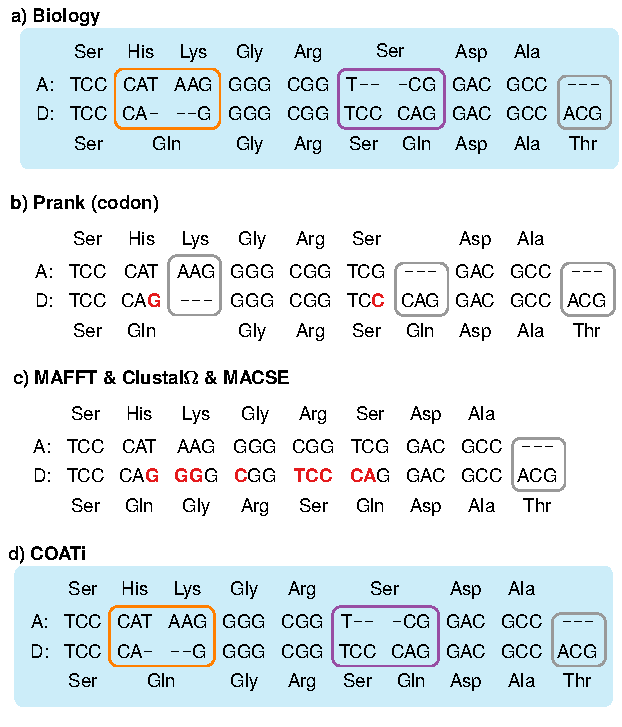
\includegraphics[scale=1]{fig-aln.pdf}
    \par
    \caption{
        Standard algorithms produce suboptimal alignments.
        (a) shows a possible alignment of an ancestor sequence (A) and a descendant sequence (D).
        (b), (c), and (d) are the results of different aligners.
        Nucleotide mismatches are highlighted in red. Phase 0, phase 1, and phase 2 indels are shown in gray, purple, and orange, respectively.
        Additionally, the orange indel is type II (an amino-acid indel plus an amino-acid change) while the purple indel is type I (an amino-acid indel only).
        COATi is the only aligner able to retrieve the biological alignment in this example.
        }
    \label{fig:aln}
\end{figure}

Genome quality impacts conclusions drawn from comparative genomic studies, and uncorrected errors in the alignment stage can lead to erroneous results in comparative and functional genomic studies \citembethree{estimates_schneider_2009}{effect_fletcher_2010}{hubisz2011error}.
Genomes for model organisms often get refined over many iterations and achieve high quality with meticulously curated protein coding sequences.
In contrast, genomes for non-model organisms might only receive partial curation and typically have lower quality sequences and annotations.
These genomes often lack the amount of sequencing data needed to fix artifacts, including missing exons, erroneous mutations, and indels \citembe{jackman2018tigmint}.
%
When comparative and functional genomics studies include data from non-model organisms, care must be taken to identify and manage such artifacts; however,
current alignment methods are ill-equipped to handle common artifacts in genomic data, requiring costly curation practices that discard significant amounts of information.
To address this problem, we present COATi, short for COdon-aware Alignment Transducer, a pairwise statistical aligner that incorporates codon substitution models and is robust to artifacts present in modern genomic data.

